\documentclass[a4paper,12pt]{article}

\usepackage[english,russian]{babel}
\usepackage{cmap}
\usepackage[T2A]{fontenc}
\usepackage[utf8]{inputenc}
\usepackage{amsmath}
\usepackage{multirow }
\usepackage{pgfplots}
\usepackage{wrapfig}
\usepackage{graphicx}
\graphicspath{{./images/}}
\usepackage{caption}
\usepackage{subcaption}
\usepackage{longtable}
\usepackage{xcolor}
\usepackage{ gensymb }
\usepackage{ dsfont }
\usepackage[unicode, pdftex]{hyperref}
\hypersetup{colorlinks,
	pdftitle={The title of your document},
	pdfauthor={Your name},
	allcolors=[RGB]{0 0 245}}


\textwidth=7.3in % ширина текста
\textheight=10in % высота текста
\oddsidemargin= -0.5in % левый отступ(базовый 1дюйм + значение)
\topmargin= -0.5in % отступ сверху до колонтитула(базовый 1дюйм + значение)


\begin{document}
	
	\begin{titlepage}
		\begin{center}
			{\large МОСКОВСКИЙ ФИЗИКО-ТЕХНИЧЕСКИЙ ИНСТИТУТ (НАЦИОНАЛЬНЫЙ ИССЛЕДОВАТЕЛЬСКИЙ УНИВЕРСИТЕТ)}
		\end{center}
		\begin{center}
			{\large Физтех-школа Радиотехники и Компьютерных Технологий}
		\end{center}
		
		
		\vspace{4.5cm}
		{\huge
			\begin{center}
				{\bf Вопрос по выбору}\\
				Плазма из винограда
			\end{center}
		}
		\vspace{2cm}
		\begin{flushright}
			{\LARGE Автор:\\Хамаш Виктория Насеровна \\
				\vspace{0.2cm}
				Б01-302}
		\end{flushright}
		\vspace{7.5cm}
		\begin{center}
			Долгопрудный 2024
		\end{center}
	\end{titlepage}

	\section{Введение}
	Один из самых популярных опытов с микроволновой печью - получение плазмы из винограда. Если разрезать виноград на две половинки, но оставить их соединенными кожурой и разогреть их в микроволновой печи, то можно увидеть разряды плазмы.
	\section{Теоретические сведения}
	
	\subsection*{Принцип работы микроволновой печи} 
    \begin{wrapfigure}[15]{r}{7cm}
		\centering
		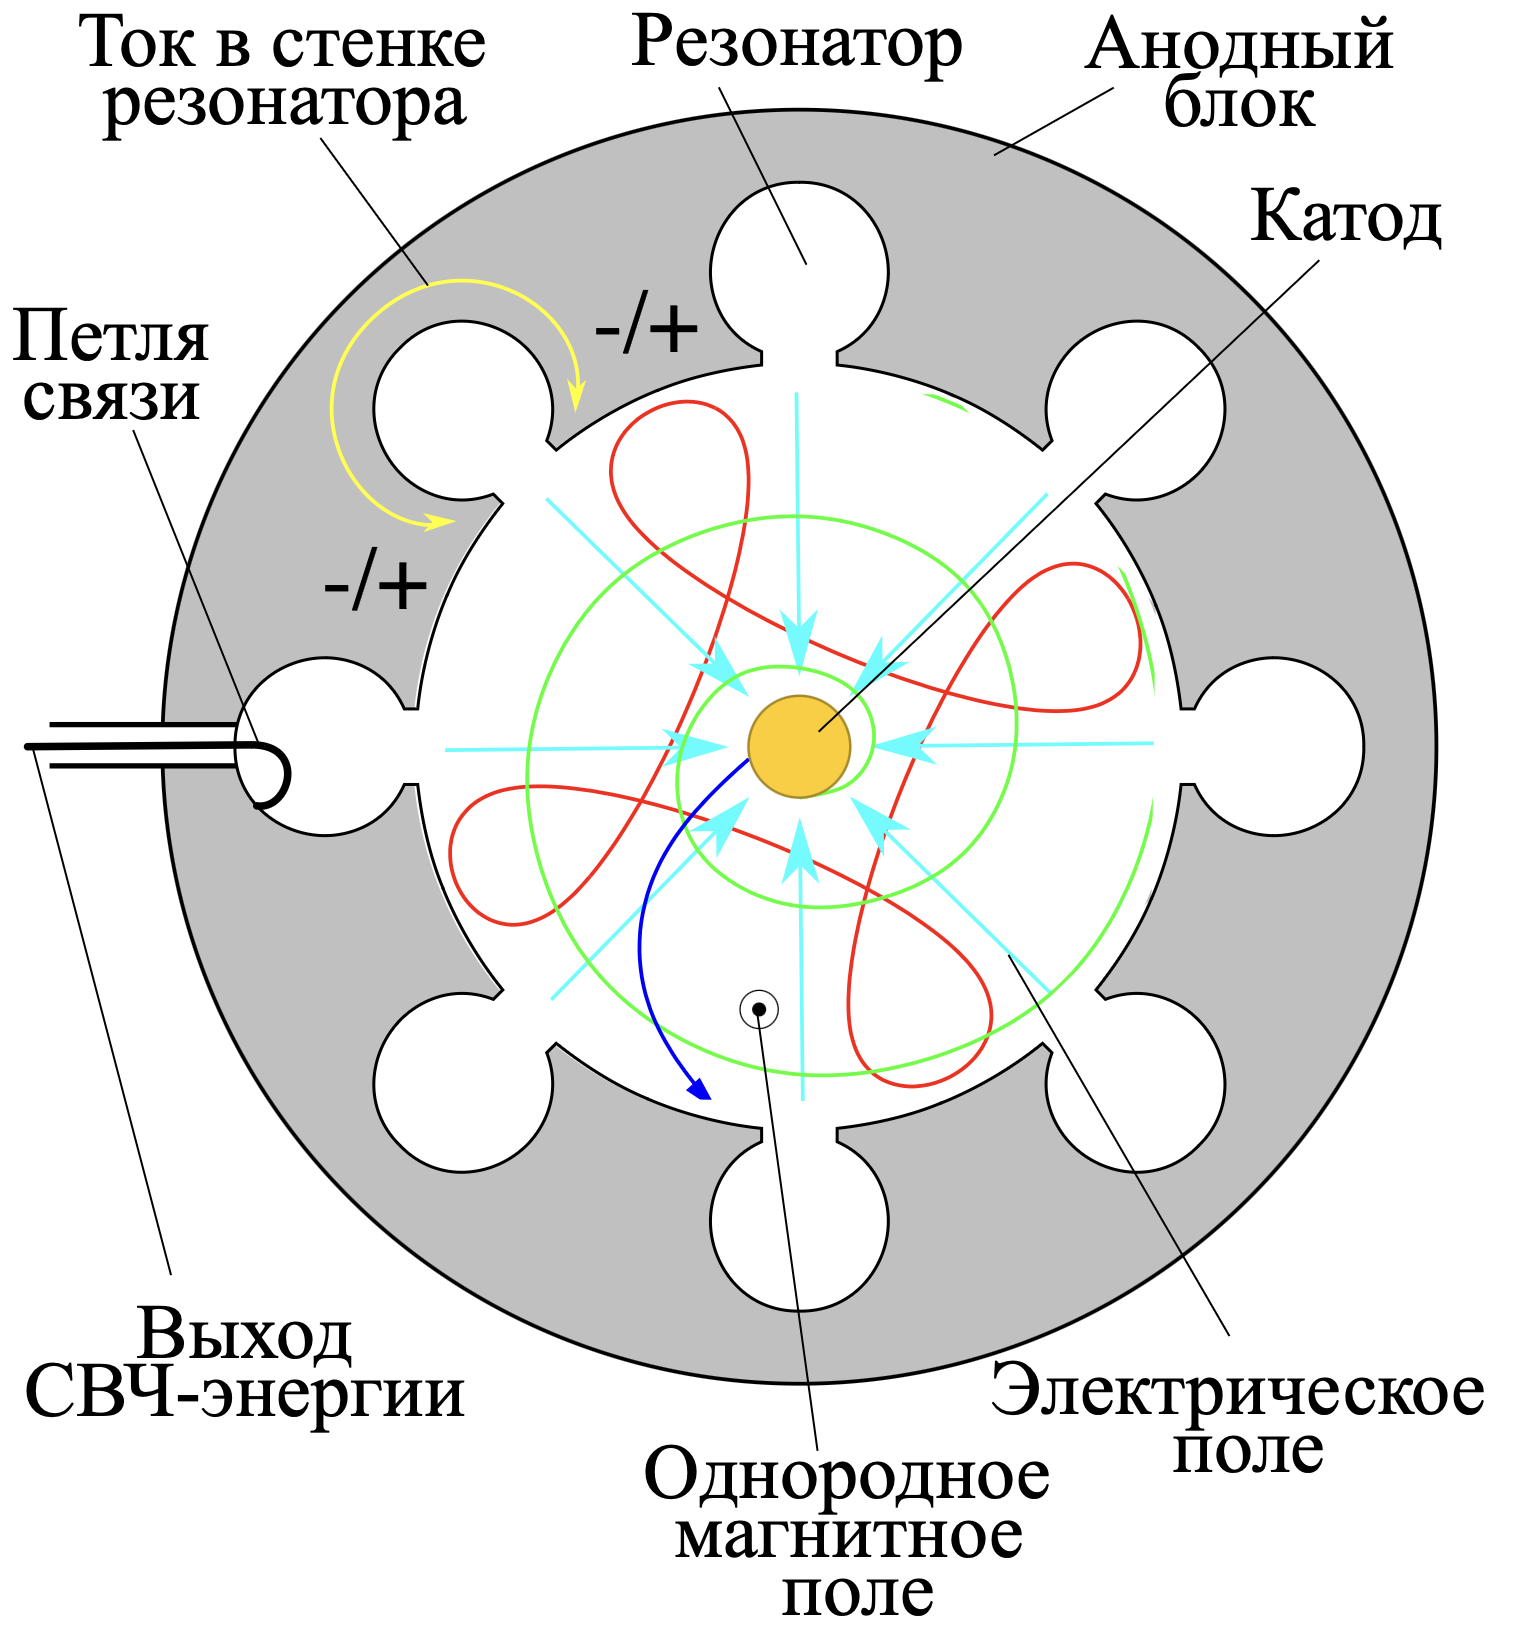
\includegraphics[scale=0.2]{magn}
		\caption{Схема магнетрона}
	\end{wrapfigure}
	\\ Основная часть микроволновой печи - магнетрон, генерирующий электромагнитные волны на частоте 2,45 ГГц. Он состоит из цилиндрического катода и анодного блока. На катоде происходит процесс эмиссии электронов: катод с помощью тока нагревается, в следствии чего начинает излучать электроны. Электроны увлекаются электростатическим полем катода и летят к аноду. Снаружи стоит постоянный магнит, который закручивает траектории электронов. В аноде вырезаны отверстия специальной формы, которые служат резонаторами. В итоге электроны пролетая мимо резонаторов своим полем возбуждают в резонаторах электромагнитные волны, которые через антенну выводятся непосредственно в печь.
	\\ \subsection*{Объяснение эффекта c виноградом}
	\\ Виноград почти полностью состоит из воды, поэтому в расчетах будем считать его таковой. Согласно \cite{litlink1} диэлектрическая и магнитная проницаемости воды при температурах $20 - 60 \ \degree C$ равны: 
	\begin{equation}
		\varepsilon \approx 79 \ \ \ \mu \approx 1.25 \ \ \ \Rightarrow \ \ \ n = \sqrt{\varepsilon \mu} \approx 9.93
	\end{equation}
	Далее посчитаем длину волны СВЧ излучения в воде:
	\begin{equation}
		\lambda_0 = \dfrac{2\pi}{k} = \dfrac{2\pi v}{2\pi f} = \dfrac{v}{f} = \dfrac{c}{nf} = \dfrac{3\cdot10^{10}}{9.93 \cdot 2.45 \cdot 10^{9}} \approx 1.23 \ cm
	\end{equation}
	То есть если виноградина будет размером примерно $\lambda_0$, то внутри её образуется стоячая волна, а значит виноградина будет нагреваться из центра наружу, а не наоборот. 
	\begin{figure}[h!]
		\centering
		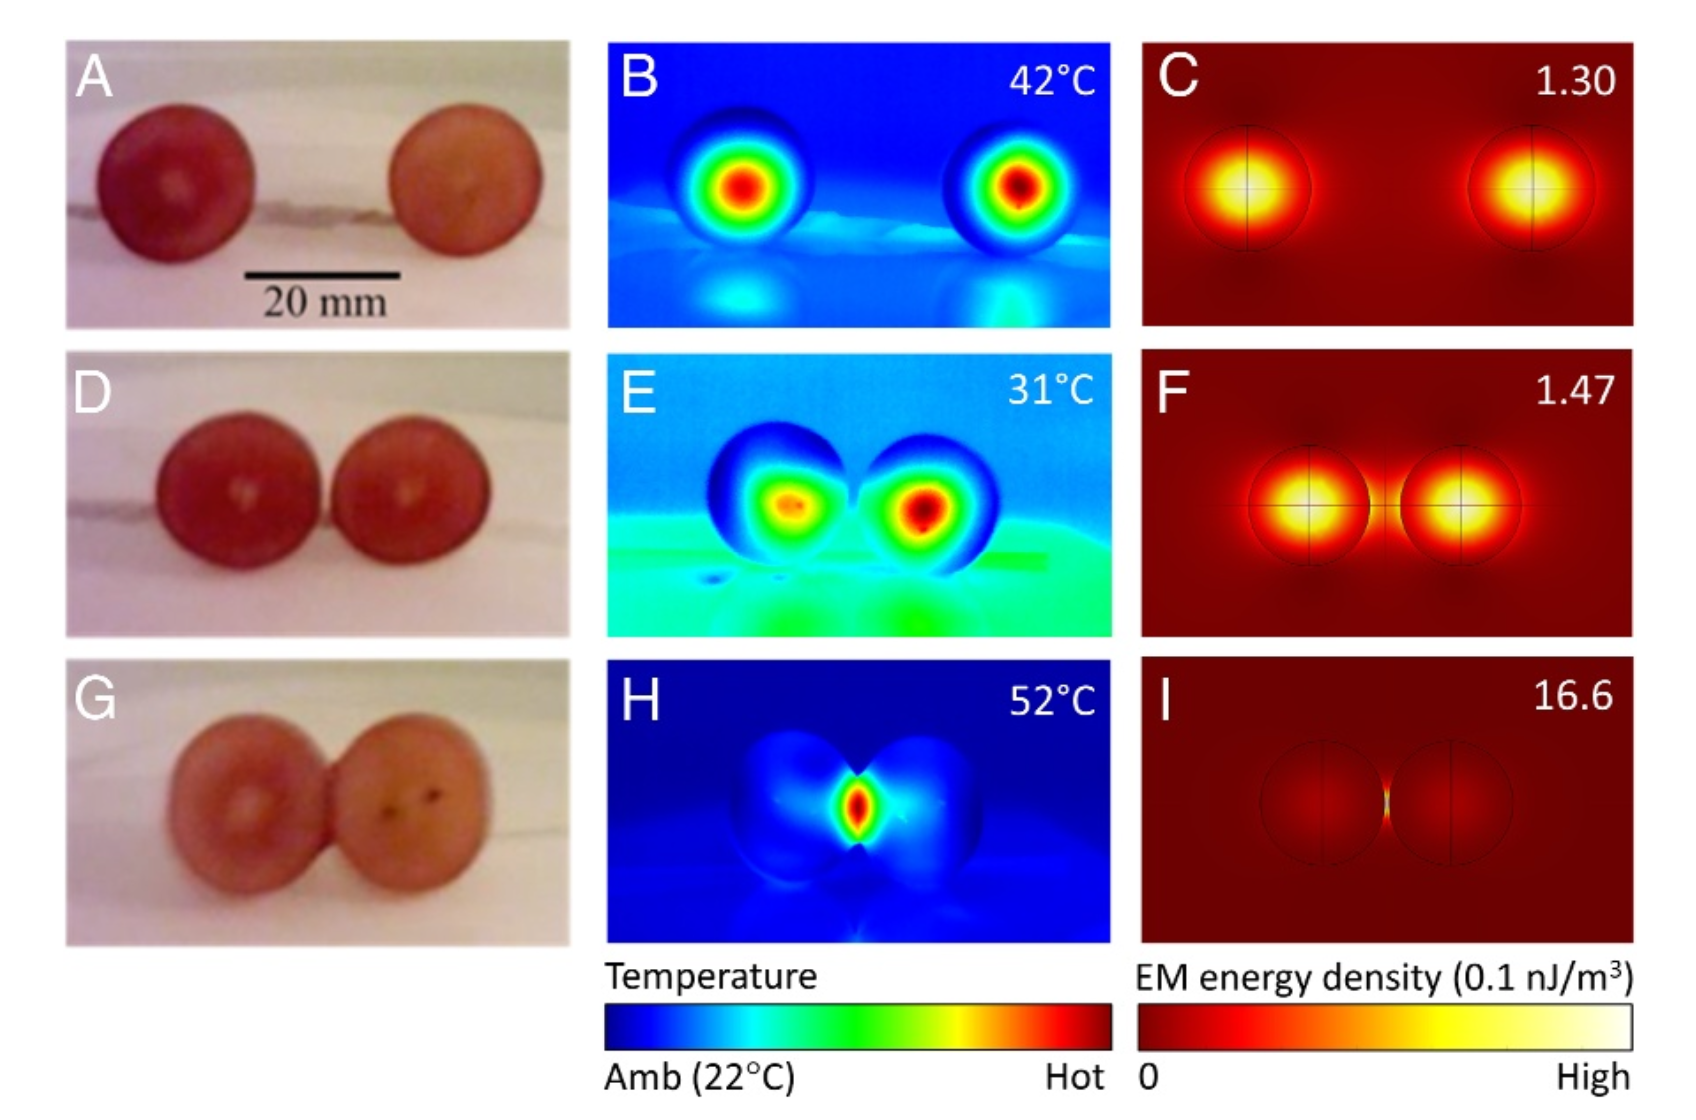
\includegraphics[scale = 0.355]{art}
		\caption{Распределение температуры внутри виноградин при нагреве СВЧ излучением из \cite{litlink1}}
	\end{figure}
	
	Также это означает, что если поставить рядом две виноградины, то в точке их соприкосновения будет пучность, а значит при достаточно мощность воздух будет ионизироваться, и мы сможем увидеть плазму. 
    \\ \\ \\ \\ \\
	\section{Оборудование}
	Микроволновая печь, излучающая на частоте 2.45 ГГц, мощностью 700 Вт; тепловизор; виноград 3 разных сортов
	\section{Эксперимент}
	Для начала возьмем одну виноградину и поместим её в микроволновую печь, как ожидалось она просто нагрелась и лопнула. Если поместить две половинки на расстоянии, то произойдет тоже самое. Но если положить две виноградины впритык или разрезать виноградину на две половины, скрепленные кожурой, то внезапно появляется плазма. В дальнейшем будем проводить опыт над одной разрезанной виноградиной, так как две виноградины спустя какое-то время отлетают друг от друга.  Положим разрезанную пополам виноградину и измерим зависимость времени до появления плазмы от  удвоенного диаметра. Измерения проводились с помощью видеокамеры телефона и ПО для видеомонтажа.
	
	\begin{table}[!ht]
		\centering
		\begin{tabular}{|l|l|l|l|l|l|l|l|l|l|l|l|}
			\hline
			$L, \ cm$ & 2.4 & 2.5 & 2.7 & 2.5 & 2.6 & 3.3 & 3.5 & 3.6 & 4.3 & 4.6 & 5.4  \\ \hline
			$t, \ s$ & 1.96 & 1.93 & 1.14 & 2.00 & 1.26 & 1.93 & 6.85 & 2.05 & 4.82 & 6.18 & 7.98 \\ \hline
		\end{tabular}
	\end{table}
	\begin{figure}[h!]
		\centering
		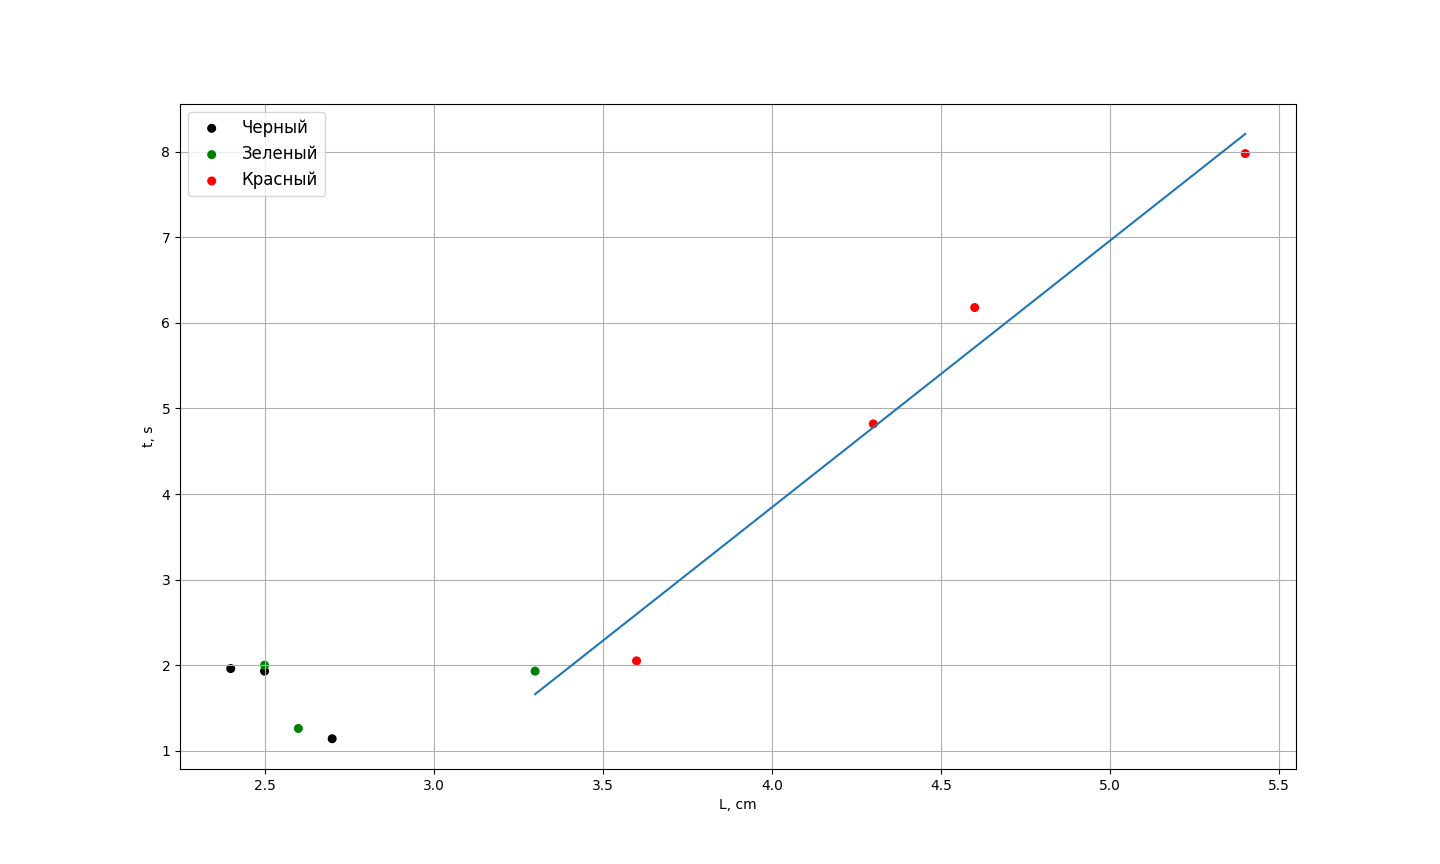
\includegraphics[scale = 0.5]{vino}
		\caption{$t(L)$}
		\label{cylcat}
	\end{figure}
	Эксперимент проводился на винограде 3 различных сортов. Видно, что зависимости от сорта нет. Минимум при диаметре виноградины $1.35 \ cm$, что соответствует оценке длины волны в воде (отклонение скорее всего связано с наличием в винограде других веществ, кроме воды). Последние 5 точек хорошо ложатся на прямую (погрешность по МНК $ \sim 7 \%$). Так как мы нагреваем тонкий кучек кожуры, то его толщина практически не изменяется, а площадь увеличивается $\sim r^2$. И так как мощность СВЧ печи остается постоянной,значит, что эффективная мощность увеличивается $\sim r^2$, а количество теплоты, которое необходимо для нагрева $\sim r^3$,  итого получается линейная зависимость. 
	
	\section{Вывод}
	В работе были рассмотрены принцип работы магнетрона, объяснение эффекта появлении плазмы при разогревании СВЧ волнами. Также были проведены эксперименты с виноградом, которые подтверждают теорию.

	
		
	% даём указание на включение данного место в оглавление как секции (\section)
	\addcontentsline{toc}{section}{Список используемой литературы}
	
	%далее сам список используевой литературы
	\begin{thebibliography}{}
		\bibitem{litlink1}  Hamza K. Khattaka, Pablo Bianuccib, Aaron D. Slepkova \textit{Linking plasma formation in grapes to microwave resonances of aqueous dimers}
	\end{thebibliography}
	
\end{document}
